\documentclass[aoas,preprint]{imsart}

\RequirePackage[OT1]{fontenc}
\RequirePackage{amsthm,amsmath}
\RequirePackage{natbib}
\RequirePackage[colorlinks,citecolor=blue,urlcolor=blue]{hyperref}
\usepackage{graphicx}
\usepackage{color}

% settings
%\pubyear{2005}
%\volume{0}
%\issue{0}
%\firstpage{1}
%\lastpage{8}
\arxiv{arXiv:0000.0000}

\startlocaldefs
\numberwithin{equation}{section}
\theoremstyle{plain}
\newtheorem{thm}{Theorem}[section]
\endlocaldefs

\begin{document}
\newcommand{\andyc}[1]{[{\color{red}\sc Andy comment: {\tt #1}}]}

\begin{frontmatter}
\title{Eliciting Mixture Priors for Assessing Fox Mortality during Fox Hunting Trials\thanksref{T1}}
\runtitle{Fox Mortality}
%\thankstext{T1}{Footnote to the title with the ``thankstext'' command.}

\begin{aug}
\author{\fnms{Andrew} \snm{Hoegh}\thanksref{m1}\ead[label=e1]{ahoegh@vt.edu}},
\author{\fnms{Ian} \snm{Crandell}\thanksref{m1}\ead[label=e2]{ian85@vt.edu}}


\thankstext{t1}{Some comment}
\runauthor{Hoegh \& Crandell}

\affiliation{Department of Statistics, Virginia Tech\thanksmark{m1}}

\address{Department of Statistics, Virginia Tech\\
Hutcheson Hall 401-D\\
Blacksburg, VA 24061\\
\printead{e1}\\
\phantom{E-mail:\ }\printead*{e2}}

\end{aug}

\begin{abstract}
Fox penning is a highly controversial practice whereby foxes are hunted with dogs in a large enclosed space. While there are commonalities with traditional horseback fox hunting, there are definite differences as well. The main difference is that with fox penning there is no chance for the fox to escape the enclosure. Using data from a fox enclosure in Virginia, we investigate the factors that influence a fox's chances to survive in such pens. In particular, a Bayesian hierarchical model is formulated to compute fox survival probabilities based on a fox's time in the enclosure and the number of dogs allowed in the enclosure. This is complicated by missing information on the number of dogs. We elicit expert knowledge for a prior on the number of dogs in a Bayesian framework to account for the uncertainty in the missing data. We then use our model to examine possible changes to fox penning policy and what effect those changes may have on fox survival. We conclude that by either allowing the foxes to acclimate to their environment or by limiting the number of hunting dogs in the pen, we can improve fox survival.
\end{abstract}

\begin{keyword}
\kwd{Survival Analysis}
\kwd{Missing Data}
\kwd{Bayesian Modeling}
\end{keyword}

\end{frontmatter}

\section{Introduction}
Fox penning is a highly charged practice, both in Virginia and nationally. This procedure is different than traditional fox hunting and government regulated hunting in general. Fox pens are enclosures that contain live foxes in which hunters bring dogs for training or sport. The controversy with fox enclosures revolves around the concept of \emph{fair chase} \citep{posewitz} and more broadly of ethics of the hunter. The Boone and Crockett Club defines fair chase as: `the ethical, sportsmanlike, and lawful pursuit and taking of any free-ranging wild, native North American big game animal in a manner that does not give the hunter an improper advantage over such animals' \citep{boone}. Under this definition maintaining animals in enclosures for hunting or training purposes cannot satisfy the requirements of fair chase.  However, consider that \cite{posewitz} claims fair chase ``is a balance that allows hunters to occasionally succeed, while animals generally avoid being taken.'' Using this definition of fair chase, we focus on assessing fox mortality in fox pens. By identifying and controlling factors contributing to fox survival, we can help policy makers mimic the spirit of fair chase by enabling high survival rates of foxes.

As with any (politically) controversial practice, there are strong opinions on both sides of the issue. With this article we stick to objective, measurable characteristics like survival rate rather than delving into subjective assessments of ethics such as animal cruelty. With that in mind, we use data from a fox pen in Virginia to assess survival of foxes in enclosures. Specifically we focus on the effect of dogs in the pens and the time a fox has to acclimate to the new surroundings. Unfortunately, missing data are present for the number of dogs in the enclosure for some days in the study. Accounting for the uncertainty induced by missing data requires care; we use a Bayesian paradigm by eliciting expert opinion as a prior. Finally, the data are not a product of a well designed experimental trial across several fox enclosures, but rather are collected at a single site. As such, caution should be exhibit when applying results from this pen to other enclosures, both in Virginia and nationally. Nevertheless, our assessment contains data driven results for evaluating policy implications for fox penning.

The remainder of this article follows as: Section 2 outlines the data used in the study, Section 3 details our modeling approach, Section 4 describes the model results, Section 5 presents a set of hypothetical policy regimes, and Section 6 concludes with a discussion.
%%%%%%%%%%%%%%%%%%%%%%%%%%%%%%%%%%%%%%%%%%%%%%%%%%%%%%%%%%%%%%%%
\section{Data} Upon being placed in the enclosure, foxes were equipped with radio transmitters providing a way to determine the foxes survival during the study. This study contains information from 27 foxes over the course of 17 months from October 2002 to February 2004. During this time period there are two distinct types of days: trial days and non-trial days. Trial days are typically organized by hunt clubs and consist of competitions where groups of owners bring their dogs to the enclosures. On trial days there is a record of the number of dogs in the pen is available. The number of dogs ranges from 50 to 752 during the trials. Unfortunately on non-trial days the number of dogs is not available; although this does not imply that no dogs are present. On non-trial days the enclosure is open for business allowing hunters to bring their dogs for training. However, the number of dogs in the enclosure on non-trial days typically is quite small and tends to be less than fifty.

At the beginning of the study, nine foxes were placed into the pen, the remaining foxes were added throughout the study. Of the 27 foxes, 6 survive to the end of the study. Figure \ref{fig:SurvTime} contains a box plot along with points for each fox of the survival time for the foxes in the study. 
\begin{figure}[h!]
\begin{center}
\caption{Survival Time of Foxes, dots denote time in enclosure at death and 'x' denotes time in enclosure for foxes surviving the study period}
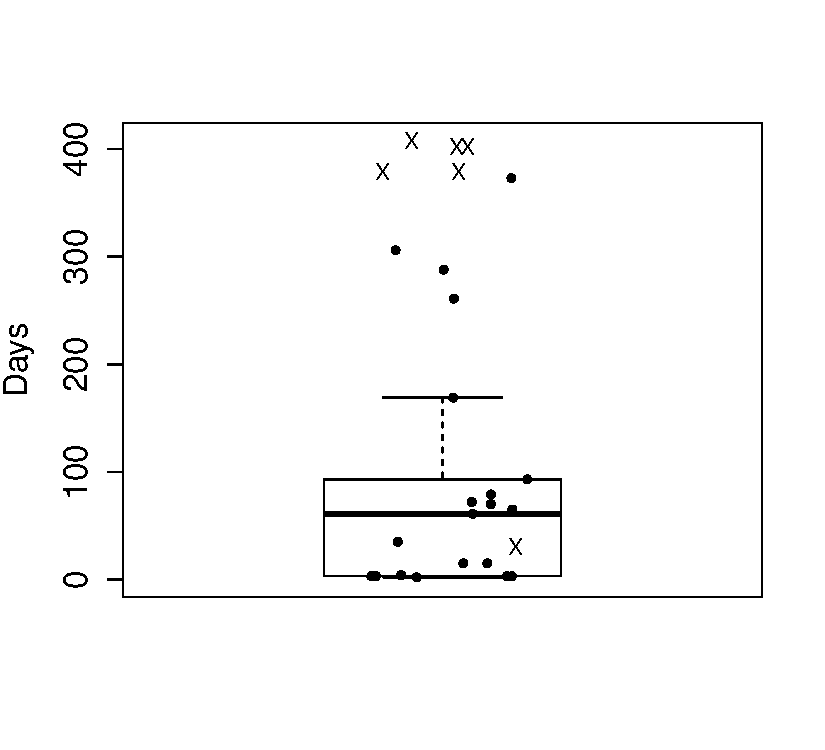
\includegraphics[width=.75\textwidth]{Survival_Time.pdf}
\label{fig:SurvTime}
\end{center}
\end{figure}
The foxes that survived to the end of the study are denoted with a `$X$'. 

For policy considerations, we consider the number of dogs in the enclosure and the time a fox has had to acclimated to the enclosure as the factors for fox survival. Obviously more dogs hunting the foxes should lower the survival rate. Acclimation time allows a fox to establish a territory and become acquainted with the area and find features that increase survival probabilities. Furthermore, the interplay between these two variables may also be important as foxes new to the enclosure on days with a large number of dogs may be particularly susceptible. 

\subsection{Missing Data}
As the number of dogs in the enclosure on non-trial days is unknown and not strictly zero, our models need to account for this. Simply using zeros (or any other constant) would fail to capture the uncertainty present in the data and lead to flawed inferences. Generally speaking this procedure is known as missing data analysis, for a comprehensive overview readers are referred to \citep{little}.  \andyc{mention types of missingness here}.

A common classical technique for dealing with missing data is multiple imputation \citep{rubin1976,rubin}. In essence, imputation is conducted several times to consider the uncertainty inherent in predicting unknown values.
From a Bayesian perspective, inferences are made from the posterior distribution of unknowns. For a covariate with missing data consider $
	\mathcal{X}=\left[
	\begin{array}{ll}
	X \\
	X^{*} 
	\end{array}
	\right]$ \\ 
	and $X^{*}$ denotes missing values for covariate $X$. Then given a prior distribution on the missing covariates, uncertainty in the missing data is accounted for in a typical Bayesian framework by integrating over the distribution \citep{boone2009}. Specifically, the posterior distribution can now be computed as $$P(\Theta|X,Y), = \int P(\Theta|X,X^{*},Y) p(X^{*}) dX^{*}.$$
	for parameters $\theta$ given data $Y$ and covariate $X$. Hence, we have a posterior distribution that accounts for the uncertainty caused by missing covariates.

\section{Model} \andyc{Typical survival models focus on expected life span, given a treatment. It is typically assumed that the treatment will have a lasting effect (beyond the time it is administered). However, in our case the treament effect is a point mass at the day it is administered. As such we model the daily survival probability}
We are concerned with policy implications for survival of foxes in enclosures and as such it is more practical to impose restrictions on daily behaviors than to consider the lifetime of a fox. Hence, we use a model for the survival of fox on a given day based on the number of dogs in the enclosure and the acclimation time of the fox. Traditional survival models such as the Cox proportional hazards model \citep{cox} or a discrete survival model were considered, but this scenario does not fit neatly into the survival framework \citep{klein} of these models. In a survival model, a treatment is given to an observational unit, the foxes in our case. However, for policy implications limiting the treatment (e.g., number of dogs) over the lifetime of a fox would be impractical, rather constructing regulations for the enclosure as a whole would be preferred. Furthermore, a lacking feature of our dataset is the age of the fox when placed in the enclosure. Without this, the interpretation of a survival model would be confusing.

Specifically a binary regression framework is invoked using a generalized linear model with a probit link function.
\begin{eqnarray*}
y_{it} &\sim& Bernoulli(p_{it}) \\
\Phi^{-1}(p_{it}) & = & \alpha + \mathcal{X}_{it}\boldsymbol{\beta} + \theta_{i} \\
\theta_{i} &\sim& N(0, \phi^{-1})
\end{eqnarray*}
where $i = \{1,...27\} $(fox), and $t= \{1,...,T\}$ (time) and $\Phi$ is a standard normal cdc function. The variable $y_{it}$ is a binary variable corresponding to survival($y_{it}=1$) or death of fox $i$ on day $t$. The matrix $\mathcal{X}_{it} = [Dogs_t\; log.exp_{it}\; (Dogs*log.exp)_{it}],$ contains the number of dogs on day $t$, the log of experience for fox $i$ on day $t,$ and their interaction. Furthermore, in line with previous notation $\mathcal{X}$ includes the missing data values for the number of dogs. The $\theta_i$ terms are random effects for each fox, which account for differences in foxes (e.g. age) that cannot be parameterized. Let $R_{it}$ be a risk matrix, where
\[
    R_{it}=\left\{
                \begin{array}{ll}
                  1 \quad \text{ if fox i is alive and collared on day t-1}\\
                  0 \quad \text{otherwise}
                \end{array}
              \right.
  \]
  For calculation of the likelihood, only elements where $R_{it}=1$ are considered. As in \cite{albert}, we use data augmentation where 
  \begin{eqnarray}
  Z_{it} \sim N( \alpha + X_{it}\boldsymbol{\beta} +\theta_{i},1)
  \end{eqnarray}
  and
\[
    Y_{it}=\left\{
                \begin{array}{ll}
                  1 \quad  Z_{it} > 0\\
                  0 \quad Z_{it} \leq 0
                \end{array}
              \right.
  \]

\andyc{Defend priors} For prior specification, we use conjugate priors: $p(\alpha) \sim N(\alpha;0,1), \boldsymbol{\beta} \sim N(\boldsymbol{\beta};0,\Sigma),$ where $\Sigma$ is a diagonal matrix scaled such that the diagonal elements, $\sigma_{ii},$ are twice the range of the data. An informative prior $Gamma(5,5)$ is placed on the precision for the random effects, $\phi$. This insures that the fox random effects are well behaved and do not drift off to $\infty$ as might be expected for foxes that survive all of their trials (particularly under a maximum likelihood paradigm). 

This analysis also requires priors on the missing data, the number of dogs on non-trial days. We elicit expert opinion to derive a mixture distribution. In particular, a prior is constructed that is a mixture of a point mass at zero with a negative binomial distribution. Hence
\begin{eqnarray}
p(X^*) = c_0 \; \delta(X^* = 0) + (1-c_0)NB(X^*; , ),
\end{eqnarray}
where the pmf for a negative binomial distribution is: 
\begin{eqnarray*}
p(k|k,r) = {k + r -1 \choose k} (1-p)^r p ^k.
\end{eqnarray*}
This prior distribution with parameters $c_0 = 0.2, p=.1.5,$ and $r=3$ can be visualized as in Figure \ref{fig:Prior}.
\begin{figure}[h!]
\begin{center}
\caption{Prior distribution on number of dogs in enclosure}
\includegraphics[width=1\textwidth]{Mixture_prior.pdf}
\label{fig:Prior}
\end{center}
\end{figure}
\andyc{finalize after getting input on prior}

\section{Results}
To fit the model we use Markov Chain Monte Carlo (MCMC), specifically a Gibbs sampler with a Metropolis inside Gibbs step for the missing data. \andyc{explain updated results here}. The sampler was run for 500,000 iterations to insure convergence for all of the parameters. The large number of iterations were necessitated for proper mixing, mostly a result of the missing data. Estimates of the coefficients and 95\% credible intervals are give in Table \ref{tab:PostEst}. The random effects parameter $\phi$ denotes (unsurprisingly) that different foxes have different survival probabilities. Furthermore, inclusion of the random effects controls for variation amongst the foxes and allows valid inferences within our model framework.
\begin{table}[h!]
	\begin{center}
		\begin{tabular}{|c|c|c|}
			\hline
			& mean & CI \\
			\hline
			$\alpha$ & 5.4 & (3.0,11.6) \\
			$\beta_{dogs}$ & -.008 & (-.015, -.004) \\
			$\beta_{exp}$ & -.65 & (-2.04,-.10) \\
			$\beta_{dogs*exp}$ & .0014 & (.0006, .0030)\\
			$ \phi$ & 0.79 & (0.07, 2.06) \\
			\hline
		\end{tabular}
		\label{tab:PostEst}
	\end{center}
	\caption{Table of model coefficients.}
\end{table}
 This shows that no credible interval contains 0, indicating that all predictors explain significant variation in survival. To visually inspect the role of the predictors we create the heat map in Figure \ref{fig:SurvProb2}.
\begin{figure}[h!]
\begin{center}
\caption{Survival Probability of Foxes as a function of experience and dogs in enclosure.}
\includegraphics[width=1\textwidth]{survivalprob.pdf}
\label{fig:SurvProb2}
\end{center}
\end{figure}
We see that fox survival is lowest when there are many dogs and inexperienced foxes. This survival rises drastically as either the number of dogs drops or the experience of the foxes increases.

\section{Policy Analysis}
\andyc{Update results:} The motivating goal of this paper was to find ways to increase the probability of foxes serving in pens. Based on our model results, we considered four hypothetical policy regimes:
	\begin{itemize}
		\item Regime A: No constraints on number of dogs or allotted acclimation time. This is currently in place.
		\item Regime B: Two weeks acclimation time with no dogs.
		\item Regime C: No more than 400 dogs allowed in pen at a time.
		\item Regime D: Two weeks acclimation time and 400 dog limit.
	\end{itemize}
Uainf these four regimes we explored the expected survival for a typical fox if it had been placed in the enclosure on October 1, 2002, the first day of the study period. For regimes (B-D), we zero out the number of dogs for the acclimation time and restrict the number of dogs to the specified limit on days where the actual number of dogs exceeded the limit.
These four regimes produced the curves in Figure \ref{fgr:1}, where the solid line represents the mean expected survival probability up to day $t$ and the dashed lines denote Bayesian credible intervals.
\begin{figure}[h]
	\begin{center}$
		\begin{array}{cc}
		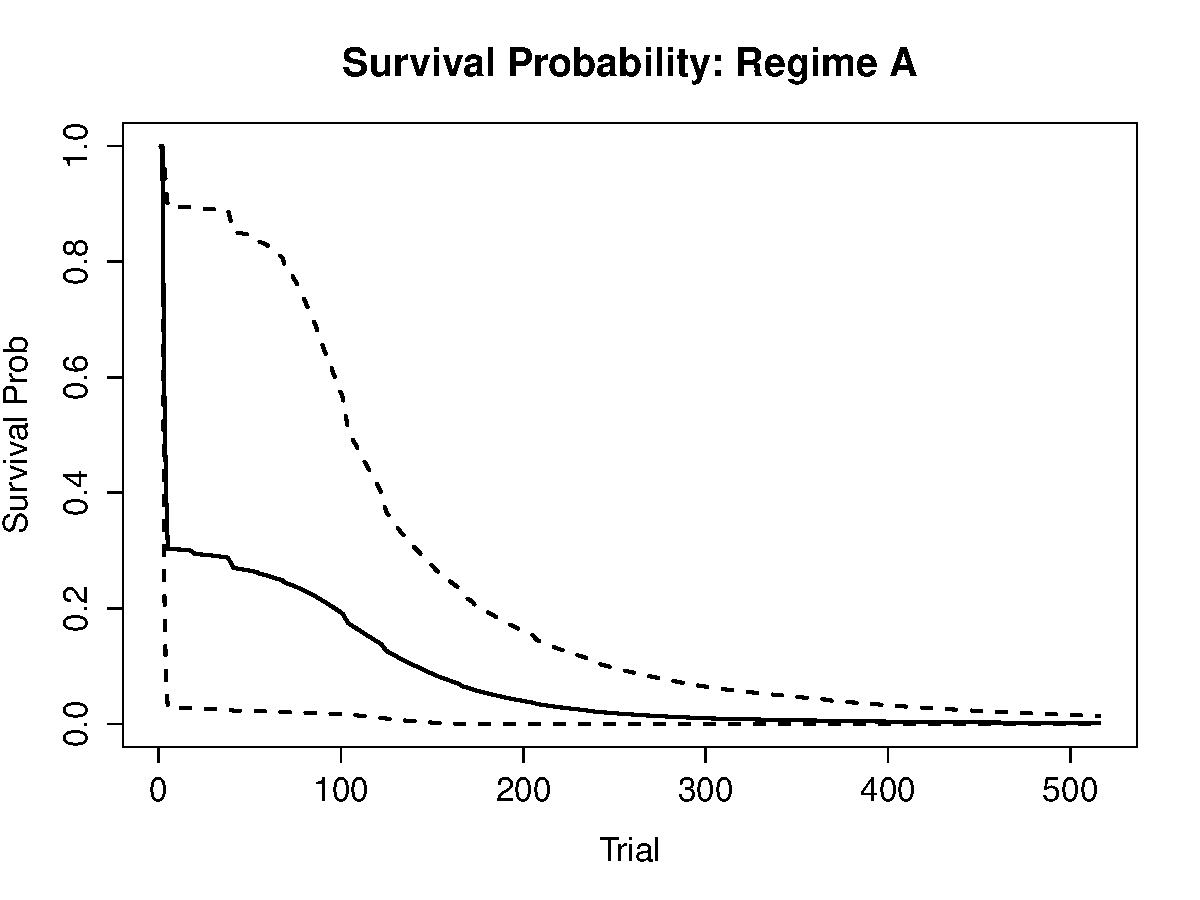
\includegraphics[width=.5\textwidth]{RegA.pdf} & 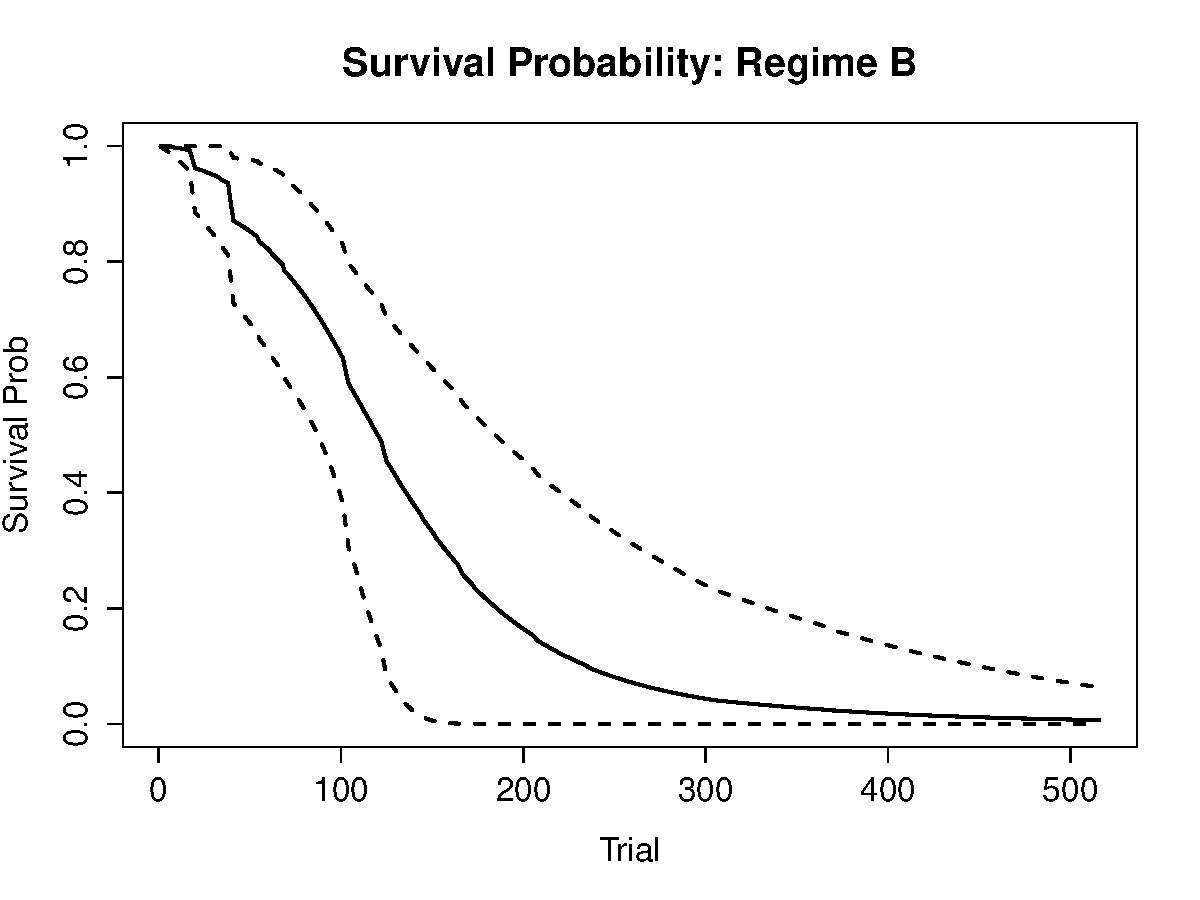
\includegraphics[width=.5\textwidth]{RegB.pdf}\\
		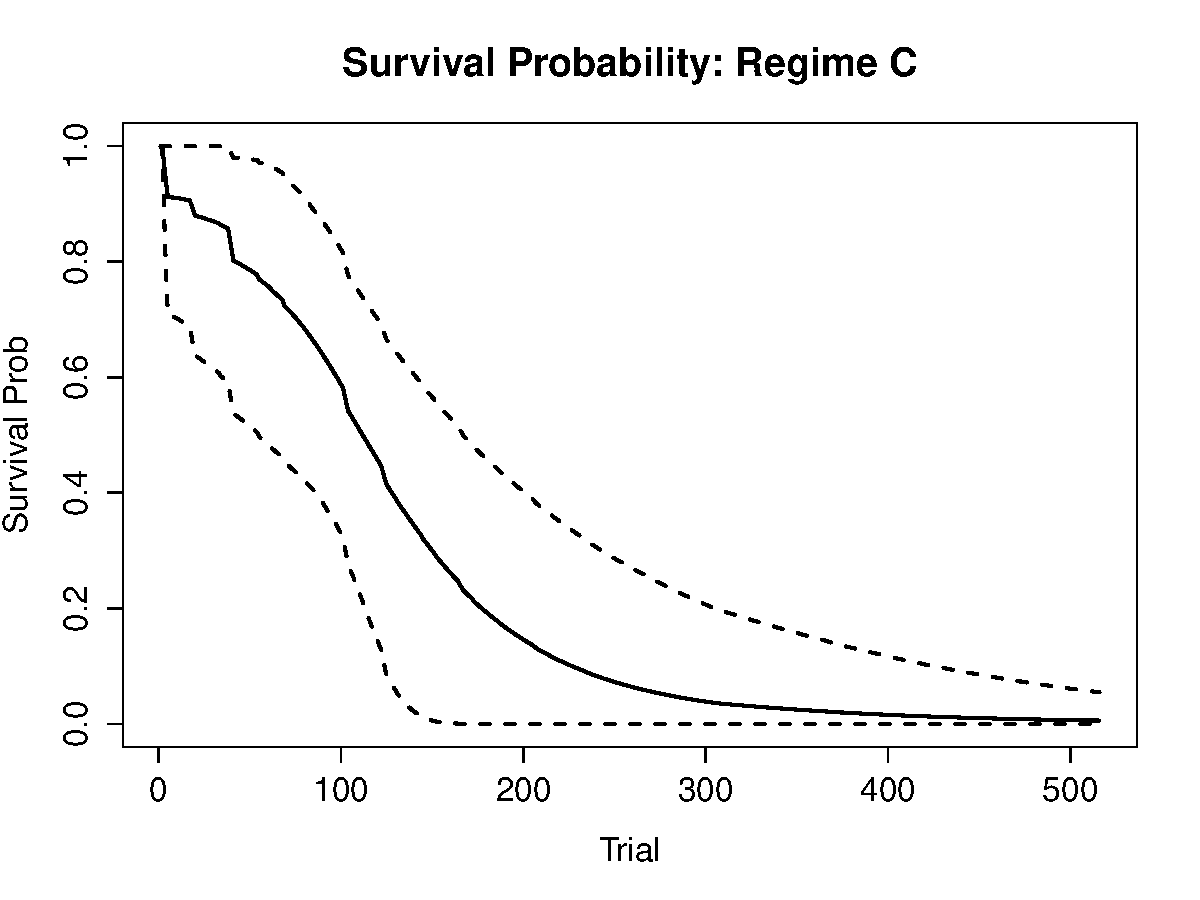
\includegraphics[width=.5\textwidth]{RegC.pdf} & 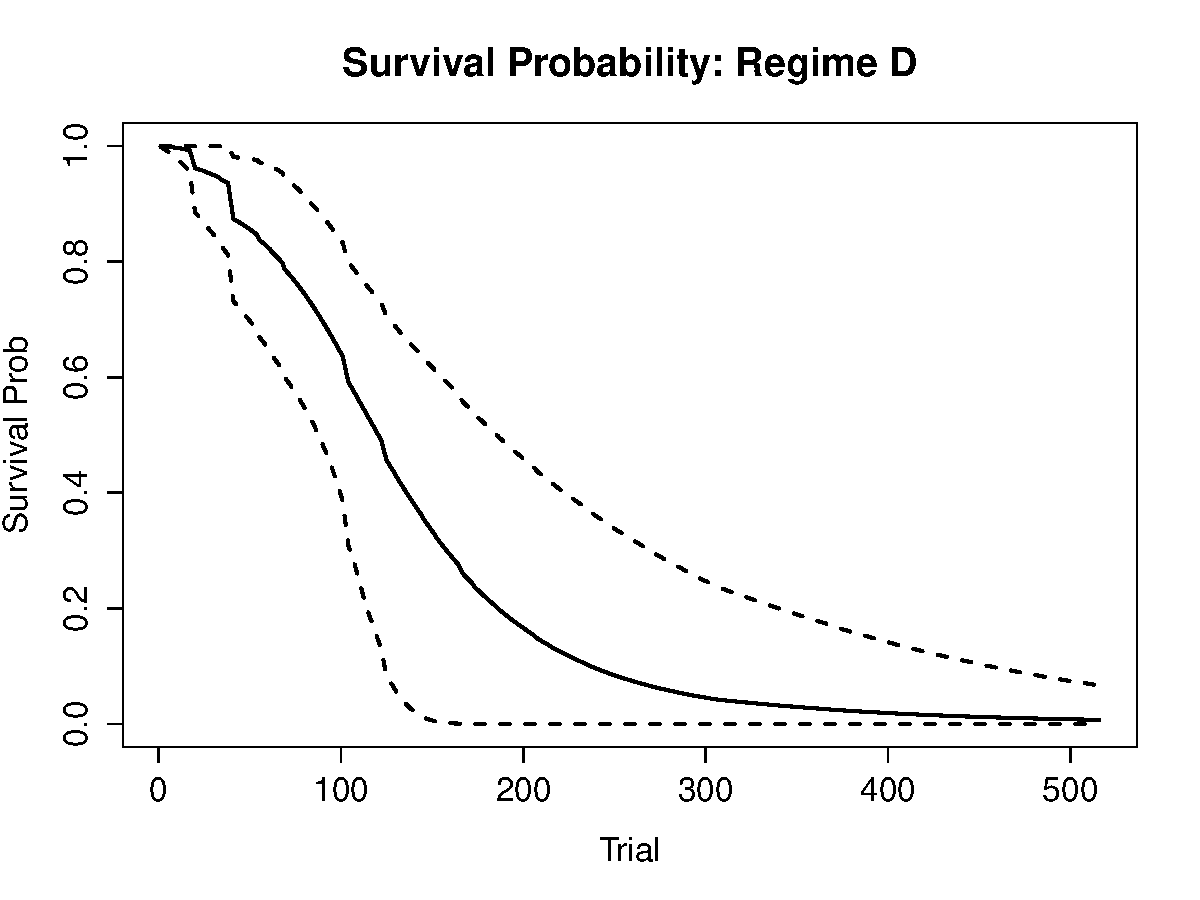
\includegraphics[width=.5\textwidth]{RegD.pdf}
		\end{array}$
	\end{center}
	\caption{Survival Probabilities for the four regimes}
	\label{fgr:1}
\end{figure}
These are not survival curves, per se, but rather the probability of a fox surviving until day $t$ given the trials conducted in the enclosure. Again, the survival rates are dependent of the number of dogs in the enclosure. We use the reported values from the trials coupled with our missing value imputation subject to restrictions for a given regime. These survival probabilities are conditioned on the number of dogs in the enclosure during the study period. This could easily be simulated to reflect other data sequences such as more or less trial days.

We see a precipitous drop in fox survival for regime A but not for any of the other three regimes. In fact, the other three plots look very similar. This accords with the heat map of survival probabilities, where we see a significant increase in survival probabilities as either the fox becomes more acclimated or the number of dogs is decreased. 

\subsection{Study Limitations}
Due to limitations in the data, it is not possible to answer some relevant questions. For instance, we cannot do a comparison of survival rates for penned versus wild foxes. In the wild, foxes generally live around five years \citep{hunter}, but we cannot compare this to penned foxes as the ages of the foxes place in the enclosure are unknown. Second, it is likely that individual characteristics of the pen contribute to fox survival and may not apply to other enclosures. Even after transforming number of dogs to dogs per acre, the results would not necessarily apply to other enclosures. Hence, caution is warranted in applying these results to other fox pens. Nevertheless, we encourage the use of any and all data for policy making; however, limitations need to be understood. Finally, a lurking variable may be the total number of foxes in the pen, which unfortunately is not available. It may be the case that a pen contains ample refuge for a given number of foxes, but beyond that number fox fatalities will be expected to increase.

\section{Discussion}
While our analysis has been about fox survival, we do not take a stand on issues of cruelty or attempt to determine an \emph{acceptable} survival rate. Our focus is strictly on factors affecting survival and we present the inferences drawn from the data. The issues of cruelty and survival are best left in the hands of policy makers.

We find that significant fox experience and the number of dogs as well as their interaction to significantly influence fox survival probabilities. In particular low levels of fox acclimation and high number of dogs are problematic. Our regime analyses reflect this fact, as fewer than half of the foxes survive beyond the first couple of days day under the current policy. Fortunately, it only takes a small change in policy to greatly improve fox survival. By either allowing the foxes acclimation time or by limiting the number of dogs in the pen we can eliminate the drastic fox mortality we see in the current regime and balance the hunters success with the foxes ability to escape.

\bibliographystyle{asa}
\bibliography{refsFox}

%\begin{thebibliography}{9}
%
%\bibitem{r1}
%\textsc{Billingsley, P.} (1999). \textit{Convergence of
%Probability Measures}, 2nd ed.
%Wiley, New York.
%\MR{1700749}
%
%
%\end{thebibliography}

\end{document}
